\section{Project Status}
\label{sec:pro-stat}

\subsection{Preliminary Work}
\label{subsec:pre-work}

The initial phase of the project consisted in handling technical aspects and 
setting up the components for the basic testbed proposed earlier 
in~\cite{Rodrigues2013b}. The following subsections briefly describe the work 
conducted during this phase.

\subsubsection{Hardware}
\label{subsubsec:hardware}

Table~\ref{tab:hw} summarizes the hardware selected for running the previously 
suggested (see~\cite{Rodrigues2013b}) test setups. Types and quantities were 
slightly altered according to the testbed arrangements on the proposal.

\begin{table}[h!]
    \centering
    \footnotesize
        \begin{tabularx}{0.75\textwidth}{ l l l X }
            %\hline
            \toprule
            \textbf{Test Element}           & \textbf{Type}                     & \textbf{Model}            & \textbf{Qty.} \\ [0.5ex]
            \midrule
            Content Source(s)               & Desktop PC (w\slash Ubuntu 12.04) & -                         & 1 \\ [0.5ex]
            \midrule
            Inner Node(s)                   & Wi-Fi Routers (openWRT~\cite{website:openwrt})   & Linksys WRT160NL~\cite{website:wrt160nl}  & 3 \\ [0.5ex]
            \midrule
            \multirow{3}{*}{End Node(s)}    & \multirow{3}{*}{Laptop (w\slash Ubuntu 12.04)}    & Dell Latitude E6430   & \multirow{3}{*}{3} \\ [0.5ex]
                                            &                                                   & Toshiba M70           & \\ [0.5ex]
                                            &                                                   & Macbook PRO           & \\ [0.5ex]
            \bottomrule
        \end{tabularx}
    \caption{Table of hardware for implementing the proposed test setup (refer 
        to~\cite{Rodrigues2013b} and Sections~\ref{subsec:ccn-thgpt},
        ~\ref{subsec:ccn-lat-load},~\ref{sec:obj-adj} for details on the 
        test setup).}
    \label{tab:hw}
\end{table}

\subsubsection{CCNx Setup}
\label{subsubsec:ccnx}

\textbf{Setting up CCNx at End Nodes (ENs):} This task 
consisted in compiling the latest release of CCNx (0.8.1) and installing it at 
the EN level. Initial tests with simple CCNx applications were conducted as an 
introduction to the platform. As the objective of the work is to monitor the 
performance of CCNx according to network parameters such as throughput, latency, 
traffic load, etc. a dedicated version of Wireshark was re-compiled to include 
a CCN packet dissector~\cite{website:ccn-wireshark}.\vertbreak

\textbf{Setting up CCNx at Inner Nodes (INs):} Testing CCNx on `real-world' 
constrained devices was a clear 
intention of this work, which differs from other 
studies (of different nature), performed in the near-past by Vahlenkamp et 
al.~\cite{Wahlisch2012, Vahlenkamp2012}. As mentioned in Section~\ref{subsubsec:hardware}, the 
chosen platform for the INs was the Linksys WRT160NL, running a Linux-based 
operating system openWRT (version 12.09). Although no CCNx packages were 
directly available to openWRT, a custom openWRT build with a CCNx package~\cite{website:ccn-openwrt} 
(version 0.7.2) designed for a different distribution --- CeroWRT~\cite{website:cerowrt} --- 
was successfully accomplished.\vertbreak

\subsection{Test 1: CCNx Throughput Analysis}
\label{subsec:ccn-thgpt}

Test 1 is now completed and did not significantly deviate from the description 
given in~\cite{Rodrigues2013b}. The main objective was to evaluate CCNx 
throughput and goodput under different conditions, on a 100 Mbps link, while 
transferring files of different sizes.\vertbreak

CCNx was tested using a file sending application --- \verb+ccnsendchunks+ --- 
and a receiving application --- \verb+ccncatchunks2+ --- which implement CCNx 
own flow control mechanism. For this purpose, CCNx was configured to run over 
UDP. The sending and receiving ends consisted in two laptops, labeled PC1 and 
PC2, connected with an Ethernet cable, with the following (different) 
characteristics (to be precised in the final document). Due to these 
differences, two rounds of tests have been conducted, one with 
PC1 as transmitter and PC2 as receiver, and vice-versa. The content used for 
exchange in the tests consisted in randomly generated data 
files of 500\,kB, 5\,MB and 50\,MB. The integrity of the transmitted files has 
been verified via an MD5 checksum, for all transfers. A special CCNx parameter 
was varied during the tests --- the chunk size $C$ --- which determines the 
amount of payload in a CCN Data packet. Values of 1024 B, 4096 B and 8192 B were 
tested.\vertbreak

The results of this test have been already processed and are displayed in the 
form shown in Figure~\ref{fig:test1} (with $F = 5$ and 50\,MB and $C = 8192$\,B. 
These are compared with a baseline consisting in a TCP exchange of the same 
files between PC1 and PC2.\vertbreak

\begin{figure}[h!]
\begin{minipage}[b]{0.5\textwidth}
    \centering
    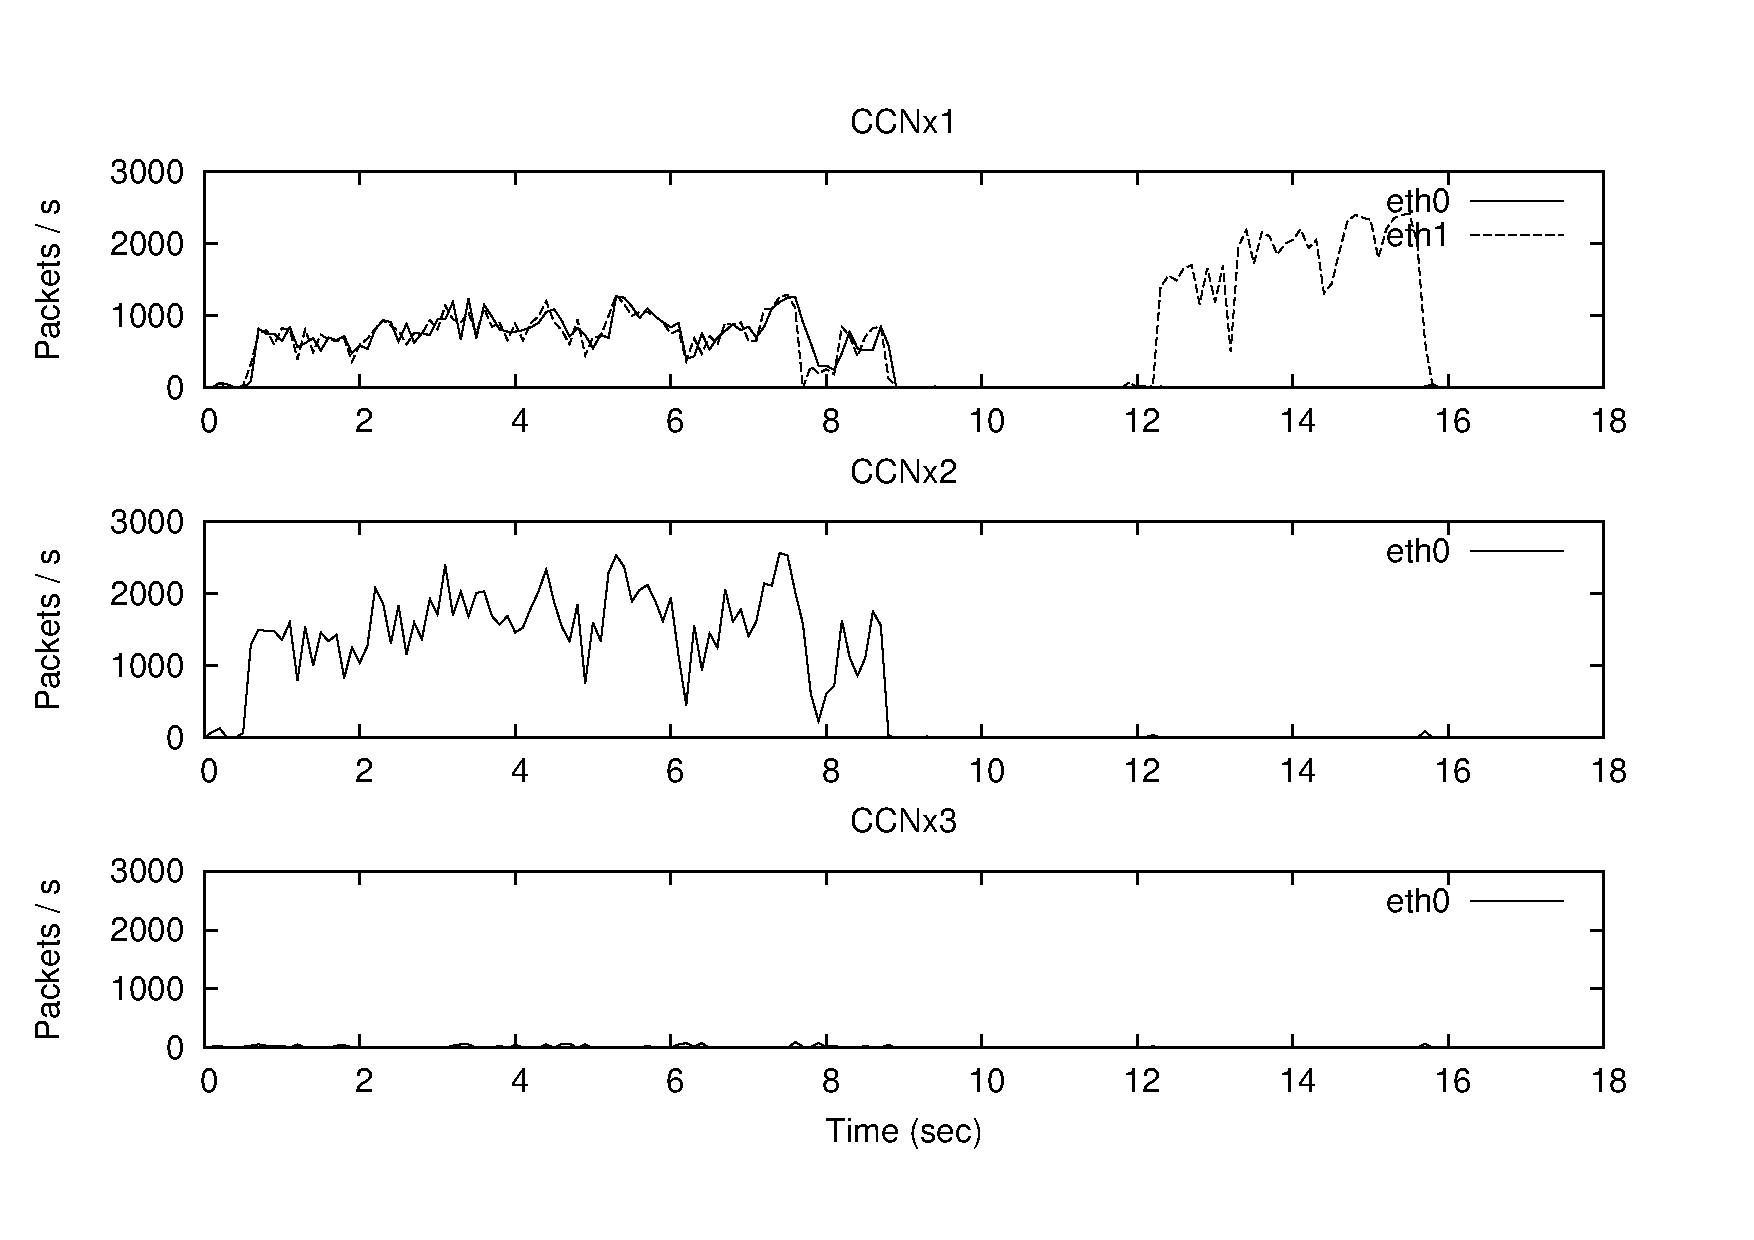
\includegraphics[width=\textwidth]{figures/long-short-route-net.pdf}
    \caption{\footnotesize Test 1 results for $F = 5$ MB, $C = 8192$ B.}
    \label{fig:subfig1}
\end{minipage}
\hspace{0.10cm}
\begin{minipage}[b]{0.5\textwidth}
\centering
    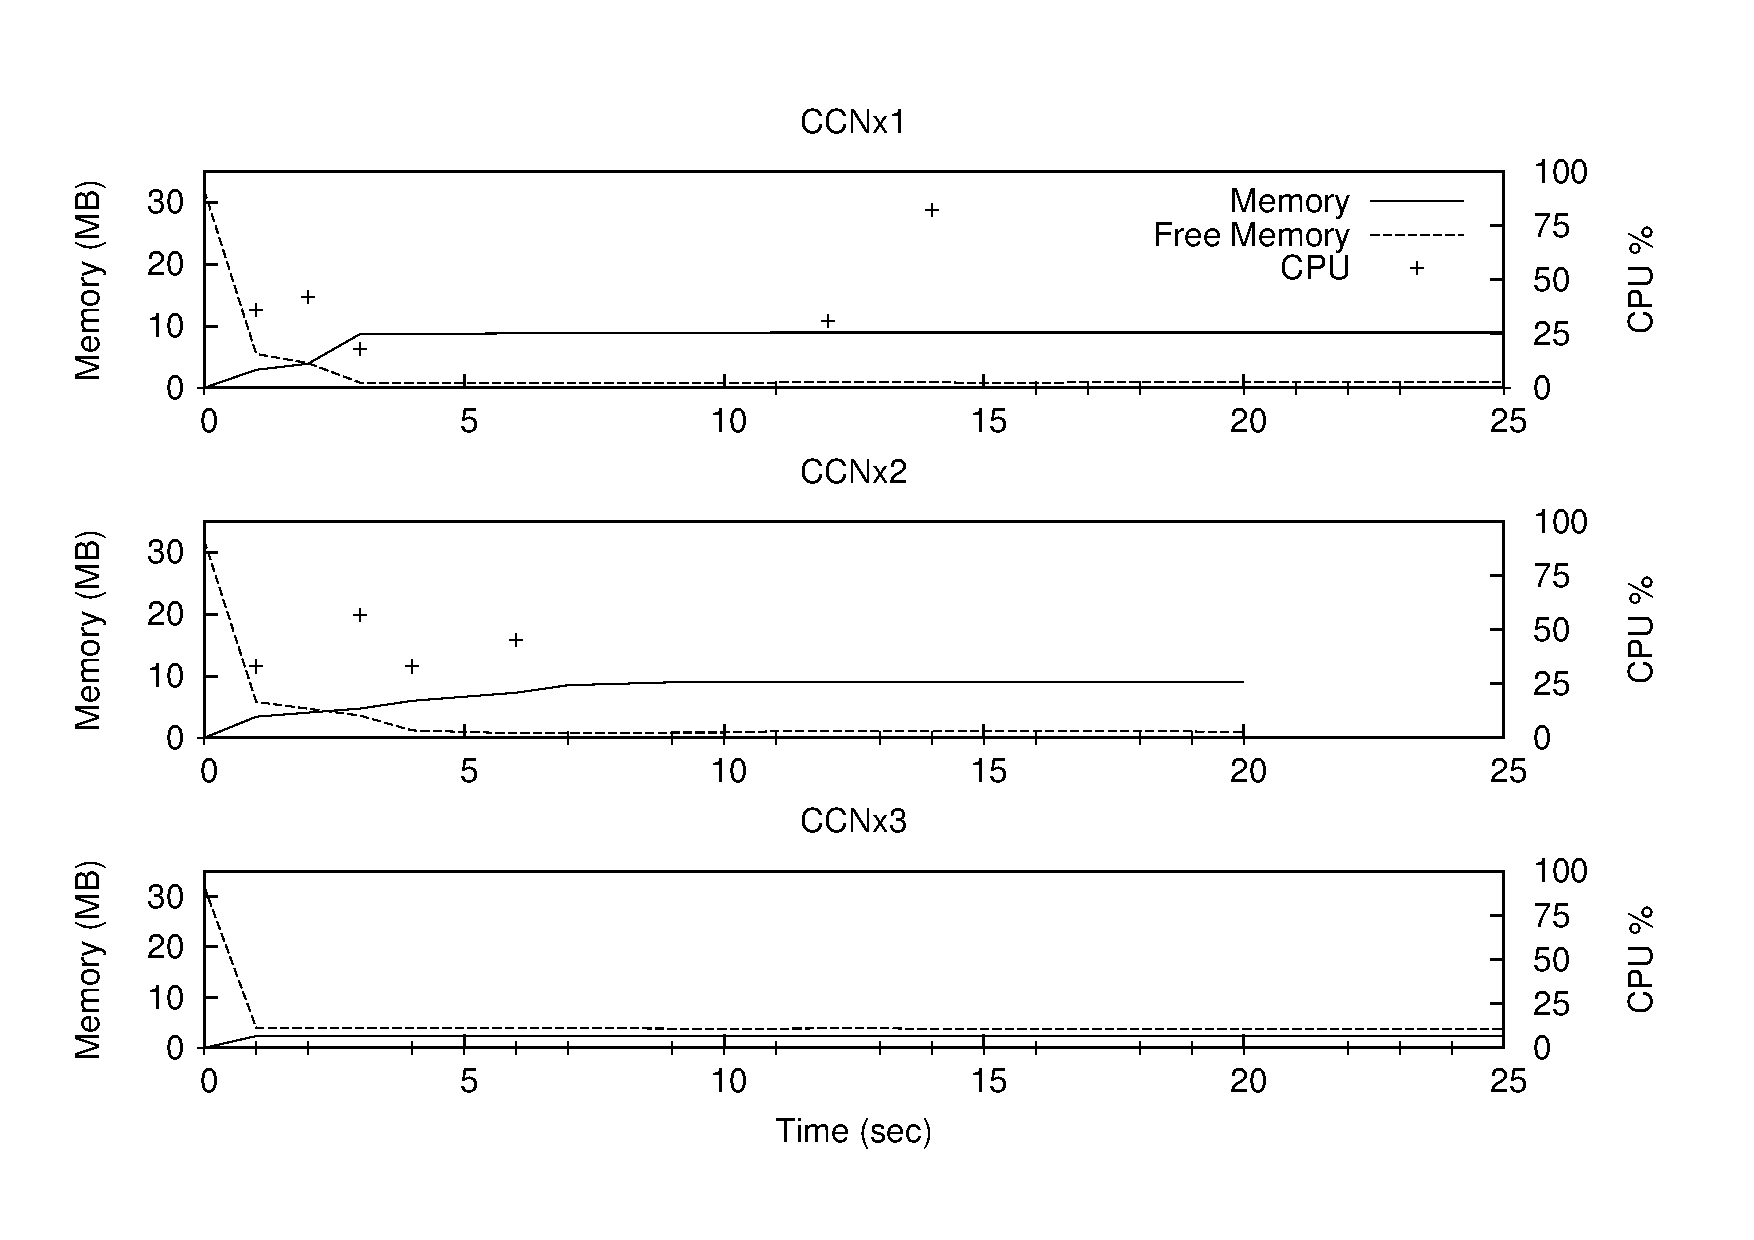
\includegraphics[width=\textwidth]{figures/file_5-long-short-route-cpu-mem.pdf}
    \caption{\footnotesize Test 1 results for $F = 50$ MB, $C = 8192$ B.}
    \label{fig:subfig2}
\end{minipage}
\cprotect\caption{Test 1 results for $F = 5$ and 50 MB, $C = 8192$ B, between 
        PC1 (receiver) and PC2 (sender). The top 
        charts provide the throughput measurement during the transfer (in Mbps), 
        and other CCNx specific parameters, as provided by the output of the 
        the \verb+ccncatchunks2+ application.}
\label{fig:test1}
\end{figure}

Data for the top chart was generated by analyzing the CCNx `flow', i.e. the 
exchange of UDP packets (with CCN's source\slash destination port number 9695) 
between the IP addresses of PC1 and PC2 using Wireshark captures and its IO 
Graph analysis. The data for the middle and bottom charts was obtained via the 
output of the \verb+ccncatchunks2+ command, which provides values for 
parameters specific to the flow control mechanism used by CCNx:

\begin{itemize}
    \item Number of Interest packets.
    \item Number of Content (Data) packets.
    \item Holes: Event which happens when a particular Data packet, for which an 
            Interest has been sent, has not arrived within a timeout. 
    \item CCNx Current Window (Curwin) size: Equivalent to TCP's window size.
\end{itemize}

The main conclusions for this test --- to be detailed on the final 
document --- are (1) the basic structure of Interest and Data packets, 
(2) the understanding of CCNx's flow control mechanism 
(which, although implementation-specific, seemed as a valid `take-home' 
lesson), (3) an experimental verification of the `one Interest per Data 
packet' concept of CCNx and (4) a comparison to a similar task performed with 
TCP.\vertbreak

\subsection{Test 2: CCNx Latency and Load Analysis}
\label{subsec:ccn-lat-load}

Test 2 is currently under evaluation (results not ready for display yet) over 
a topology similar to that shown in~\cite{Rodrigues2013b}, but with readjustments to the number 
of INs and ENs (see Table~\ref{tab:hw}). Nevertheless, the same objective remains: to 
verify how CCNx can reduce the latency when an end node $N_i$ accesses (at time 
$t + \Delta t$) content 
previously fetched from a content source $CS$ by a node $N_j$ (at time $t$), 
connected to 
the same `edge' CCN router. Besides analyzing video transmission with CCN's VLC 
plugin, the transfer of files such as in Test 1 will also be applied. In 
addition, the use of constrained devices as INs 
will allow an assessment of the feasibility of the CCN concept in LANs or other 
networks composed constrained devices.\vertbreak

